\chapter{A Classical Approach to Data Acquisition System Design}
\label{chap:III-1-arch}

  In the early development stages of the DAQ system for the GE1/1 detector, before the first version of the OptoHybrid was designed, a small prototyping setup was developed to readout a 10 cm $ \times $ 10 cm Triple-GEM detector using VFAT2 Hybrids. With time, the setup was improved to use the GLIB and later on the OptoHybrid. Next to the data readout chain, the system also controls the high voltage and gas sources from a web interface. \\

  In this chapter, we describe the evolution of the DAQ system developed to read out a small Triple-GEM prototype. We describe the technologies that have been used and the developments that were performed in order to integrate the components in the system.

  \section{The Experimental Setup}

    The experimental setup consists of a 10 cm $ \times $ 10 cm Triple-GEM detector placed between two scintillators which coincidence is used to produce triggers. The GEM prototype is equipped with a two-dimensional readout board with 2 times 128 strips in each direction. Figure \ref{fig:III-1-gem} is a photograph of the detector showing the four readout connector, the high voltage resistive divider in the bottom left, and the gas supply in the bottom right. \\

      \begin{figure}[h!]
        \centering
        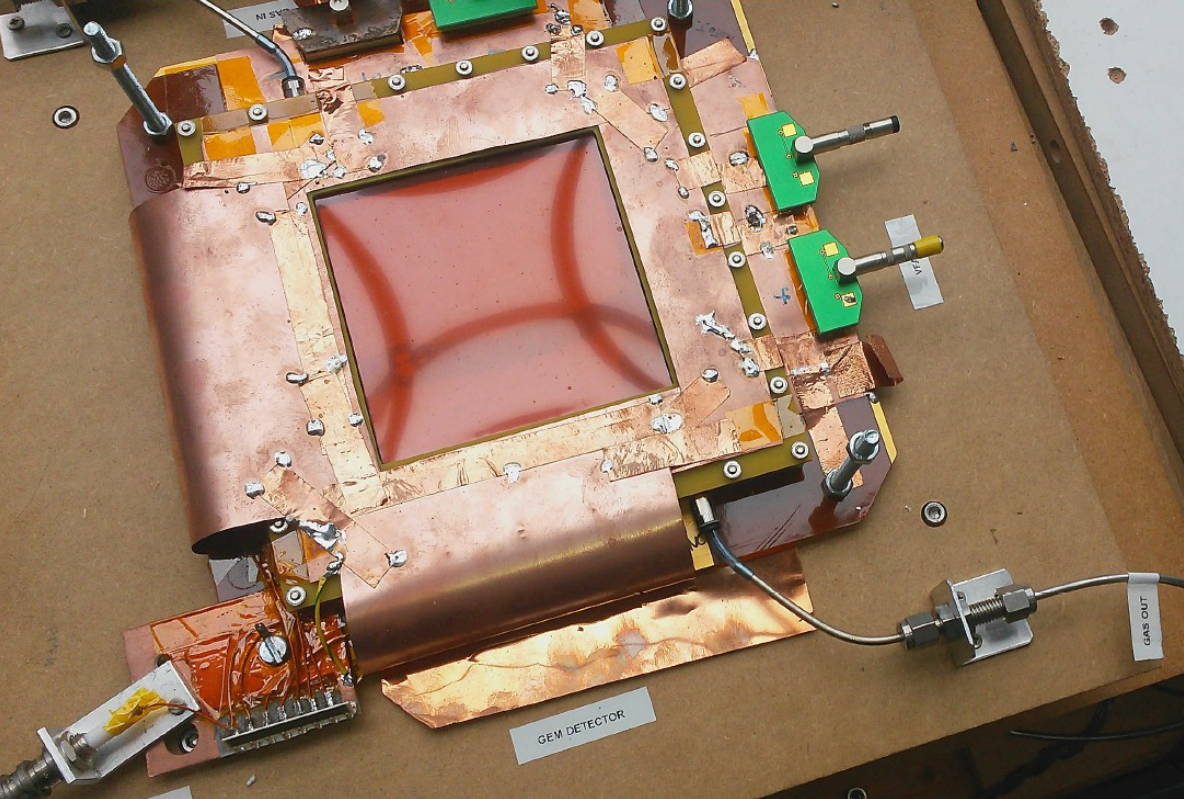
\includegraphics[width=0.8\textwidth]{img/III-1-arch/gem.png}
        \caption{}
        \label{fig:III-1-gem}
      \end{figure}

      The high voltage provided to the GEM and the photomultipliers attached to the scintillators is originating from a CAEN V6533N VME module. VME is a crate standard that defines a high speed communication protocol and an infrastructure for the interconnect of the boards. A CAEN V1718 VME-USB bridge board is used to control the communication of the VME crate from a computer. This modules allows the latter to talk to any board in the crate. The gas flow is regulated by four HORIBA STEC SEC-N112MGRW mass flow controllers: three for the Ar, CO$_2$, and CF$_4$ gas bottles and one to monitor the mixture. Figure \ref{fig:III-1-gas-hv} shows photographs of the VME high-voltage modules on the left and the mass flow meters on the right. 

      \begin{figure}[h!]
        \centering
        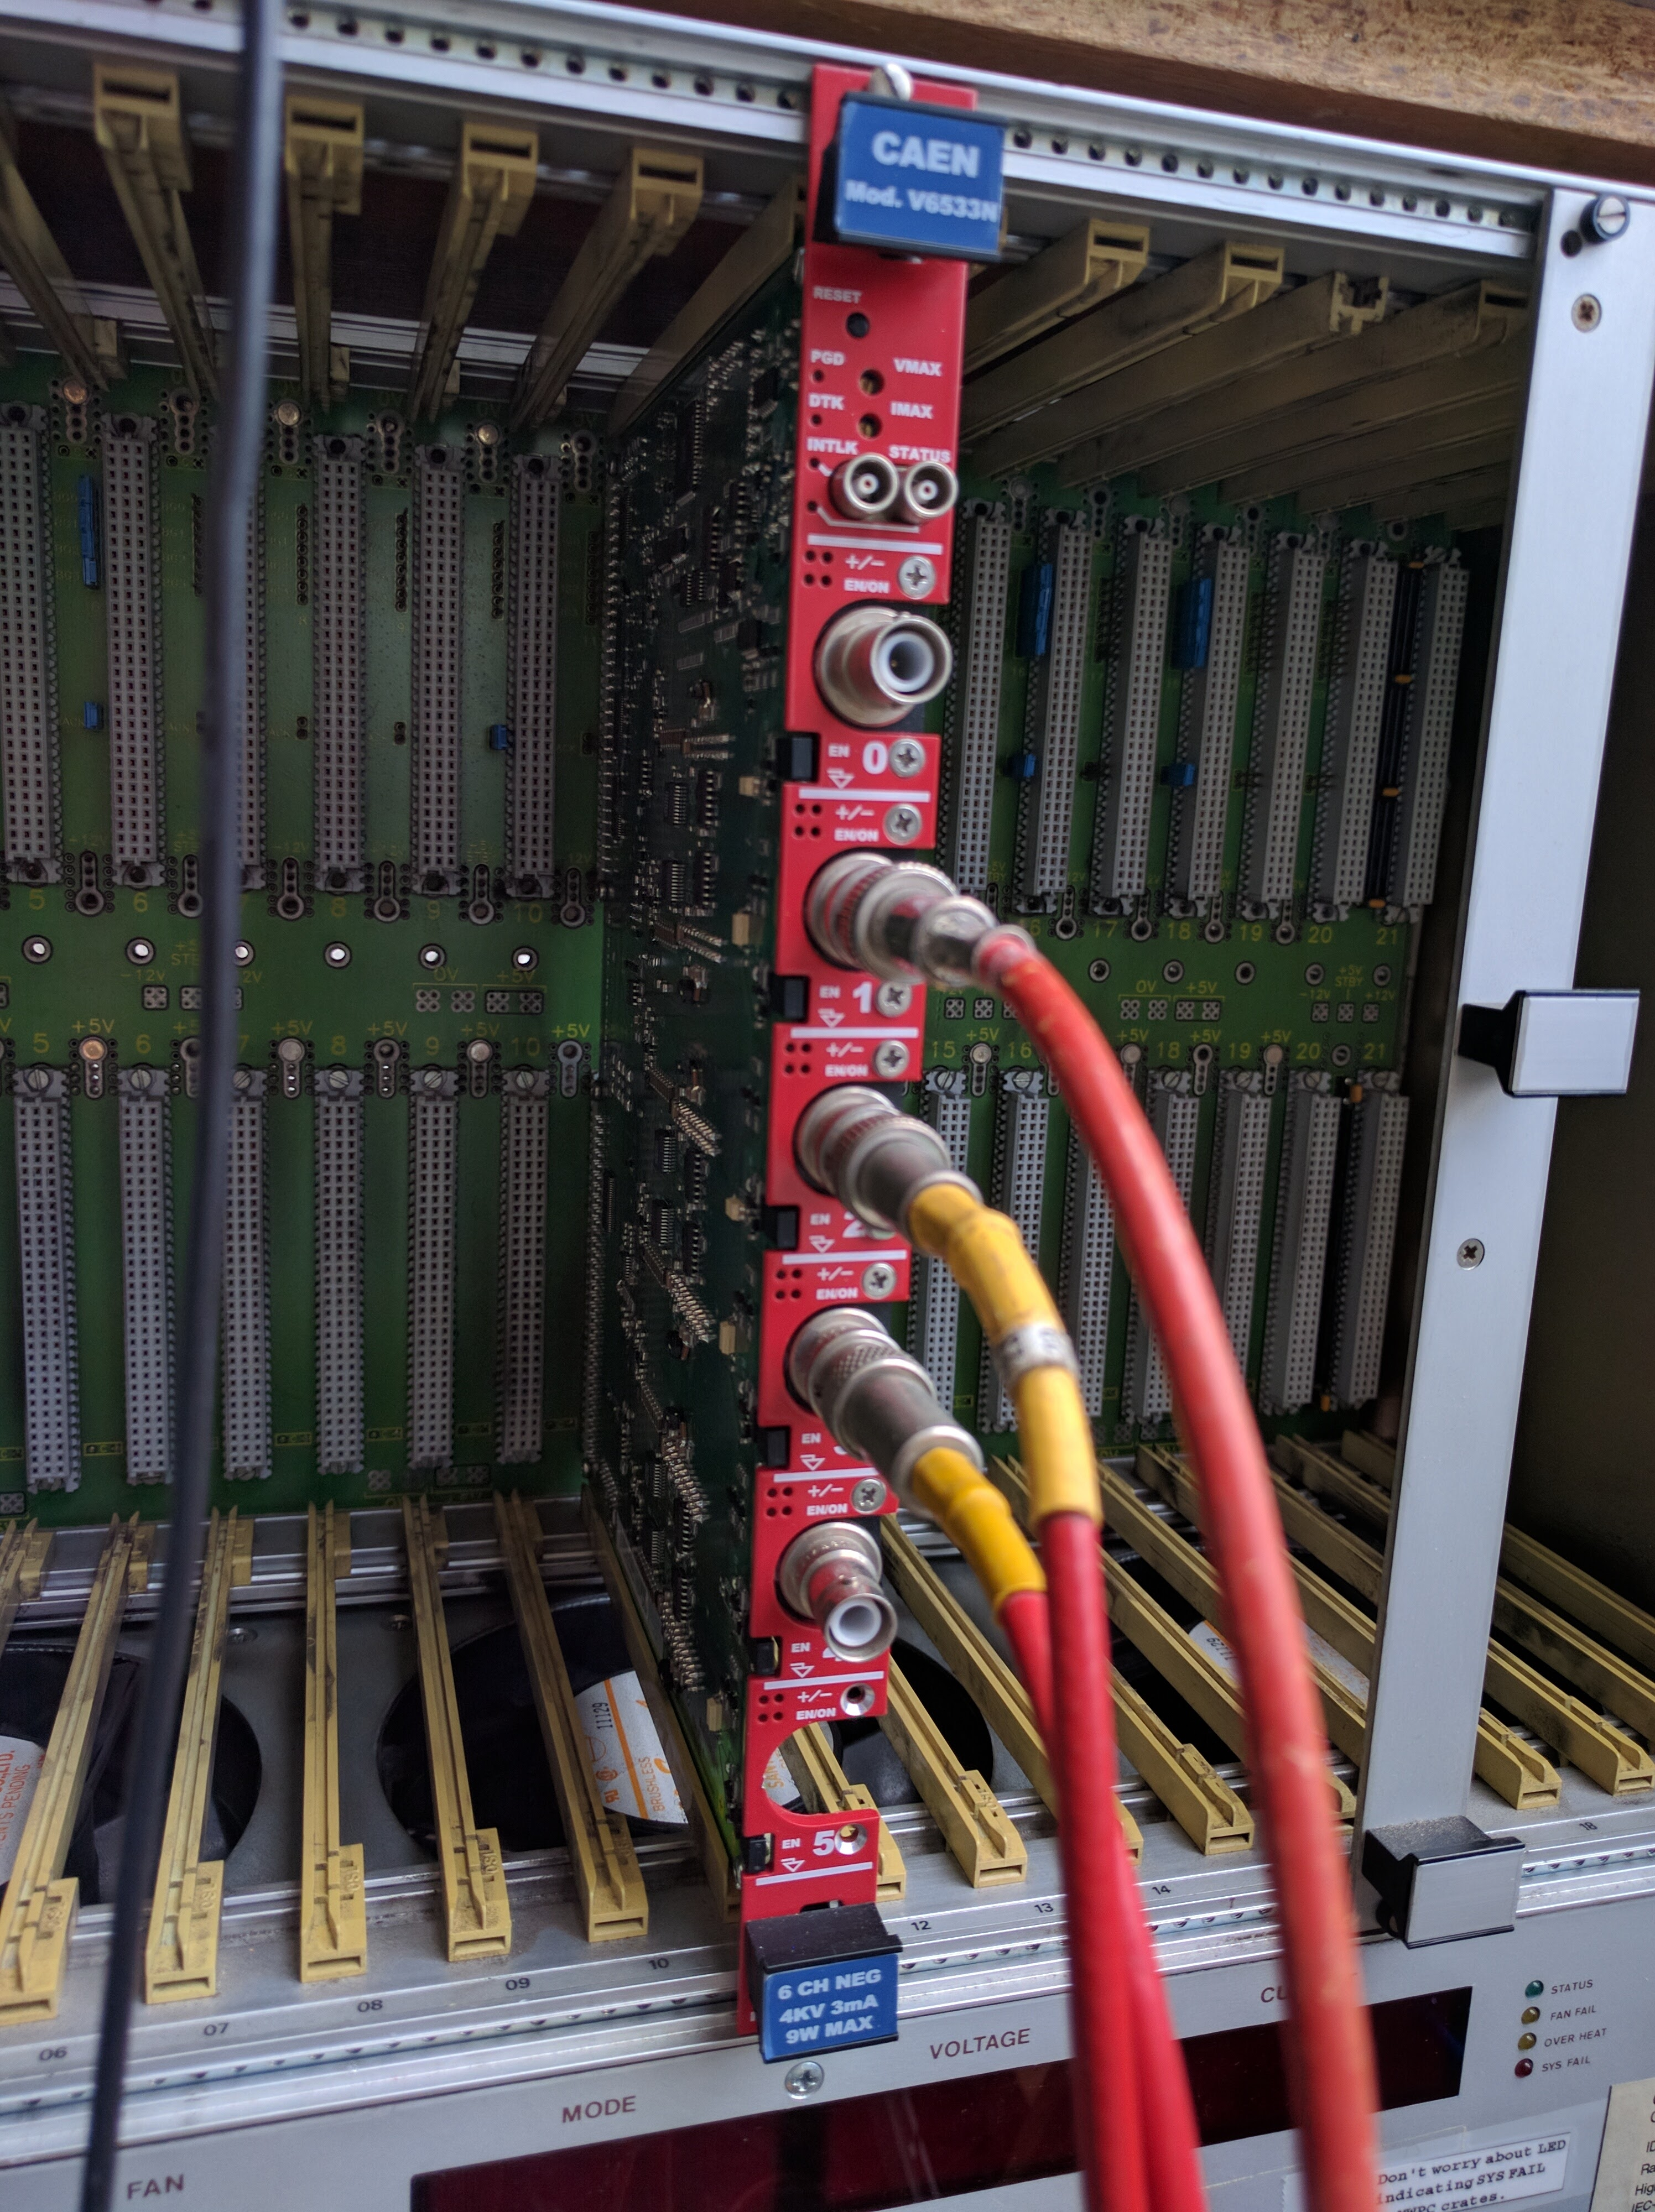
\includegraphics[width=0.39\textwidth]{img/III-1-arch/hv.jpg}
        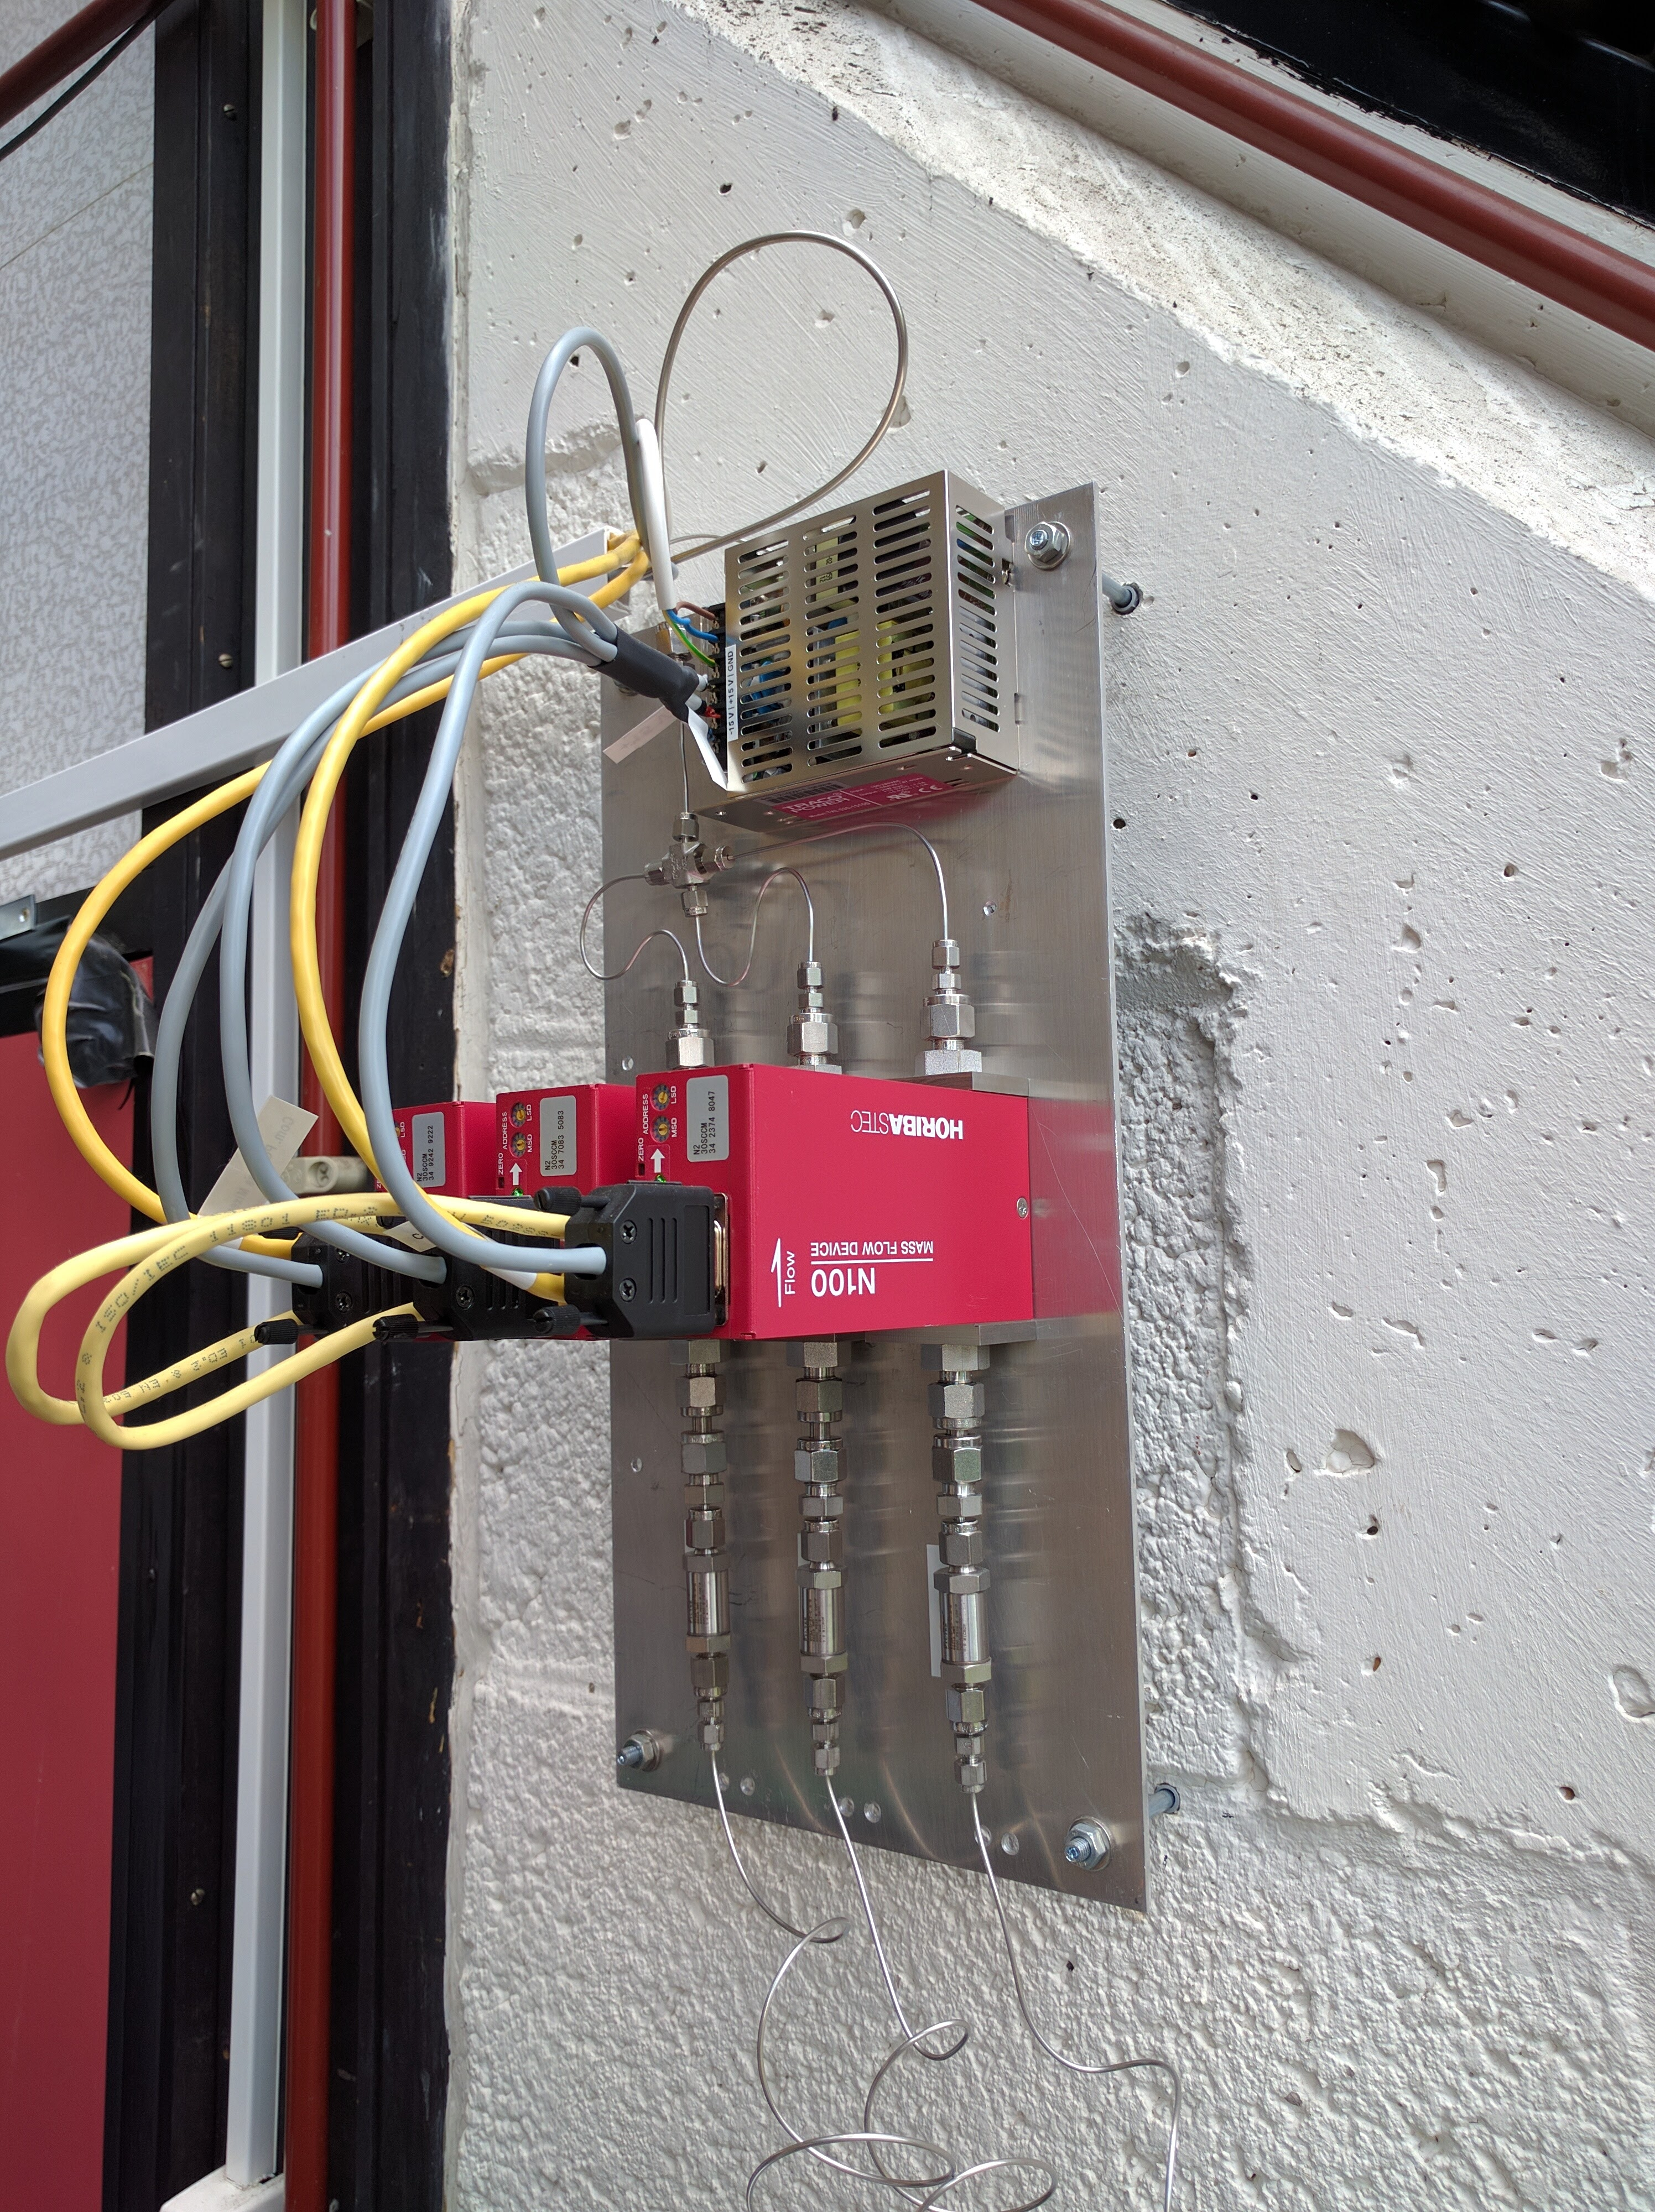
\includegraphics[width=0.39\textwidth]{img/III-1-arch/gas.jpg}
        \caption{}
        \label{fig:III-1-gas-hv}
      \end{figure}


  \section{The Infrastructure of the Data Acquisition System}

    \subsection{The Central Computing Node}

    \subsection{The Web Interface}

    \subsection{The High Voltage and Gas Controller}

  \section{A First Prototype using the Xilinx SP601 Development Board}

    \section{The MicroBlaze Softcore Processor}

    \section{IPBus over UART}

  \section{Upgrade of the System using the GLIB}

  \section{Final System using the First Prototype of the OptoHybrid}

  \section{Conclusion}
